\begin{figure}[t]
    \centering
    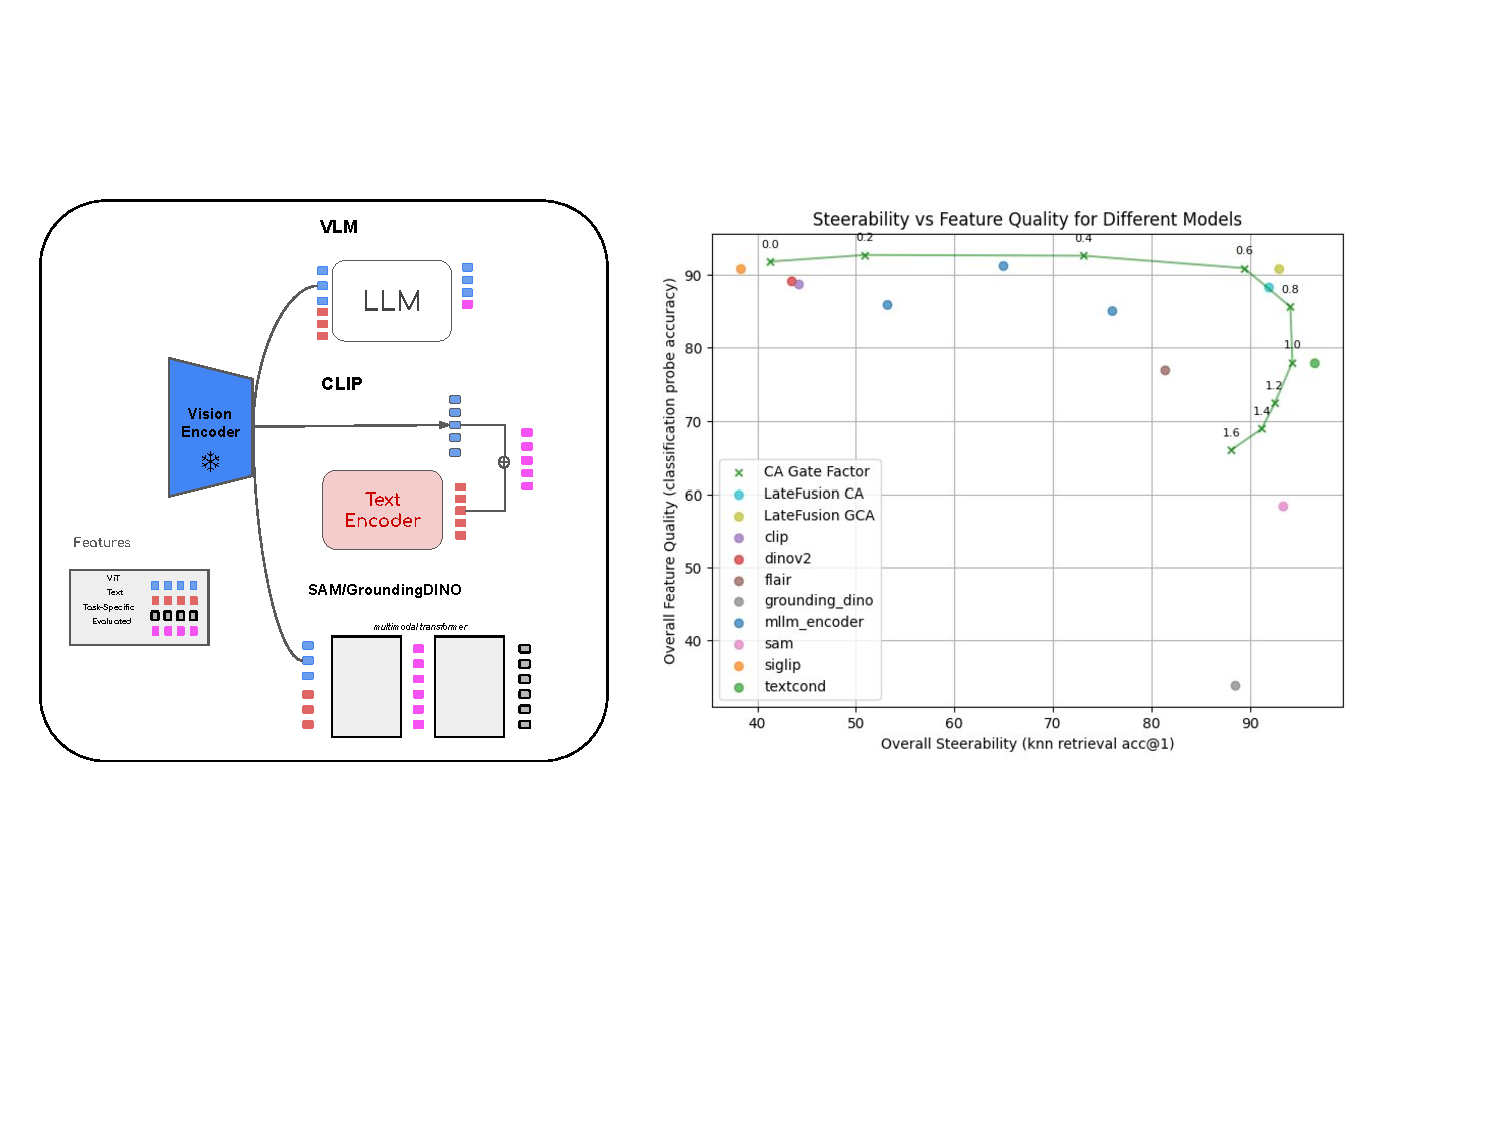
\includegraphics[width=\linewidth]{figures/teaser_3.pdf}
    \caption{\textbf{Top:} Contrasting vision-language representations with our text-conditioned visual representations.
    \textbf{Bottom:} We compare visual features along two axes - quality (global and patch level features on classification and segmentation probes) and text-steerability.
    Standard encoders (DINOv2, SigLIP) produce rich features but cannot be steered.
    Multimodal models (SAM2, GroundingDINO) are steerable but produce task-specific representations that lack generality for downstream transfer.
    SHIFT achieves both high steerability and high feature quality.}
    \label{fig:teaser}
\end{figure}

\section{Introduction}
\label{sec:intro}

Pretrained visual encoders exhibit a strong saliency bias: they effectively process images through the most prominent visual concept in the scene.
This behavior stems from photographer bias in training data, where subjects are centered and in-focus, and paired caption caption used for vision-language modelling typically describe only primary objects.
Self-attention reinforces this tendency by routing global information through high-norm tokens that correspond to salient foreground objects~\cite{caron2021dino, oquab2024dinov2}.
The result is query-agnostic representations that collapse to coarse, scene-level semantics.
Consider a kitchen image containing appliances, utensils, and a few mugs in the background: DINOv2~\cite{oquab2024dinov2} features encode the global ``kitchen,'' scene while discarding the fine-grained concepts needed to retrieve, count, or localize specific objects like the mugs.

This limitation leaves current models trapped between two extremes (Figure~\ref{fig:teaser}).
Standard visual encoders such as DINOv2~\cite{oquab2024dinov2} and SigLIP~\cite{zhai2023_siglip} produce rich, general-purpose features but offer no mechanism to focus on a particular visual concept.
Open-vocabulary localization models such as SAM3~\cite{ravi2024sam2} and GroundingDINO~\cite{liu2023groundingdino} accept text queries but produce task-specific representations that lack the generality and fidelity for downstream transfer.
No existing approach achieves both high-quality visual features and prompt-based steerability.

In this context, we explore the question: \textit{can text conditioning steer the semantics of visual representations without degrading their quality?}
We present SHIFT, a method that equips any frozen Vision Transformer with the ability to steer its features via natural language.
SHIFT interleaves tanh-gated cross-attention layers~\cite{alayrac2022flamingo} within a frozen ViT and trains them on referential segmentation, using the segmentation objective as a proxy signal to learn steerable representations.
We find that this leads to three desirable properties/desiderata:
\begin{itemize}
    \item \textbf{Global steerability:} The text query steers the semantics of the global feature vector, enabling conditional retrieval of non-salient visual concepts (\MG{vague}) in cluttered scenes (Section~\ref{subsec:cond_ret_exp}).
    \item \textbf{Dense attention routing:} Self-attention routes information through tokens corresponding to the text-described visual concept, improving localization for non-salient objects (Section~\ref{subsec:mosaic_exp}).
    \item \textbf{Feature quality preservation:} The steered representations preserve the base ViT's downstream transfer, maintaining \sout{classification and segmentation} performance on standard vision benchmarks (Section~\ref{subsec:pareto}).
\end{itemize}

Together, these properties yield a surprising consequence: text-conditioned steering generalizes to out-of-distribution domains more effectively than supervised fine-tuning.
Because our method preserves the rich visual structure learned from large-scale vision-only pretraining, natural language can focus these features on novel concepts without the catastrophic forgetting that accompanies fine-tuning on limited target data.
On personalized object discrimination, descriptive text prompts outperform a fine-tuned DINOv2 baseline in a zero-shot manner (Section~\ref{subsec:ood_generalization}).
On industrial anomaly detection, a domain entirely absent from training, our general-purpose model matches dedicated methods without any adaptation.

In summary, we make the following contributions:
\begin{enumerate}
    \item We introduce SHIFT, a text-conditioned visual encoder that instills text understanding into frozen ViTs via sparse, gated cross attention layers trained on grounding.
    % sparse, tanh-gated cross-attention layers trained on referential segmentation.
    % \item We demonstrate a Pareto improvement over existing models: SHIFT achieves high text steerability while preserving the feature quality of the underlying ViT, bridging the gap between unsteerable encoders and quality-degraded multimodal models.
    \item We demonstrate a Pareto improvement over existing models:
    % \item Our approach dynamically routes attention to task-relevant visual concepts, 
    SHIFT can guide the semantics of the visual representation with text while preserving their downstream transfer, bridging the gap between unsteerable encoders and quality-degraded multimodal models.
    \item We demonstrate that text conditioning enables zero-shot domain transfer that outperforms supervised fine-tuning: on personalized object discrimination (PODS), descriptive prompts surpass a fine-tuned DINOv2 baseline (54.4 vs.\ 48.0 PR-AUC), and on industrial anomaly detection (MVTec~AD, VisA), our general-purpose model matches dedicated methods, all without task-specific training and across ViT families (DINOv2~\cite{oquab2024dinov2}, SigLIP~\cite{zhai2023_siglip}, MAE~\cite{he2022mae}).
\end{enumerate}
